%%% Title presen0621
\documentclass[landscape,10pt]{ujarticle}
\special{papersize=\the\paperwidth,\the\paperheight}
\usepackage{ketpic,ketlayer}
\usepackage{ketslide}
\usepackage{amsmath,amssymb}
\usepackage{bm,enumerate}
\usepackage[dvipdfmx]{graphicx}
\usepackage{color}
\definecolor{slidecolora}{cmyk}{0.98,0.13,0,0.43}
\definecolor{slidecolorb}{cmyk}{0.2,0,0,0}
\definecolor{slidecolorc}{cmyk}{0.2,0,0,0}
\definecolor{slidecolord}{cmyk}{0.2,0,0,0}
\definecolor{slidecolore}{cmyk}{0,0,0,0.5}
\definecolor{slidecolorf}{cmyk}{0,0,0,0.5}
\definecolor{slidecolori}{cmyk}{0.98,0.13,0,0.43}
\def\setthin#1{\def\thin{#1}}
\setthin{0}
\newcommand{\slidepage}[1][s]{%
\setcounter{ketpicctra}{18}%
\if#1m \setcounter{ketpicctra}{1}\fi
\hypersetup{linkcolor=black}%

\begin{layer}{118}{0}
\putnotee{122}{-\theketpicctra.05}{\small\thepage/\pageref{pageend}}
\end{layer}\hypersetup{linkcolor=blue}

}
\usepackage{emath}
\usepackage{emathEy}
\usepackage{emathMw}
\usepackage{pict2e}
\usepackage{ketlayermorewith2e}
\usepackage[dvipdfmx,colorlinks=true,linkcolor=blue,filecolor=blue]{hyperref}
\newcommand{\hiduke}{0621}
\newcommand{\hako}[2][1]{\fbox{\raisebox{#1mm}{\mbox{}}\raisebox{-#1mm}{\mbox{}}\,\phantom{#2}\,}}
\newcommand{\hakoa}[2][1]{\fbox{\raisebox{#1mm}{\mbox{}}\raisebox{-#1mm}{\mbox{}}\,#2\,}}
\newcommand{\hakom}[2][1]{\hako[#1]{$#2$}}
\newcommand{\hakoma}[2][1]{\hakoa[#1]{$#2$}}
\def\rad{\;\mathrm{rad}}
\def\deg#1{#1^{\circ}}
\newcommand{\sbunsuu}[2]{\scalebox{0.6}{$\bunsuu{#1}{#2}$}}
\def\pow{$\hspace{-1.5mm}^\hspace{-1mm}$}
\def\dlim{\displaystyle\lim}
\newcommand{\brd}[2][1]{\scalebox{#1}{\color{red}\fbox{\color{black}$#2$}}}
\newcommand\down[1][0.5zw]{\vspace{#1}\\}
\newcommand{\sfrac}[3][0.65]{\scalebox{#1}{$\frac{#2}{#3}$}}
\newcommand{\phn}[1]{\phantom{#1}}
\newcommand{\scb}[2][0.6]{\scalebox{#1}{#2}}
\newcommand{\dsum}{\displaystyle\sum}

\setmargin{25}{145}{15}{100}

\ketslideinit

\pagestyle{empty}

\begin{document}

\begin{layer}{120}{0}
\putnotese{0}{0}{{\Large\bf
\color[cmyk]{1,1,0,0}

\begin{layer}{120}{0}
{\Huge \putnotes{60}{20}{インストール状況}}
\putnotes{60}{50}{高遠節夫}
\end{layer}

}
}
\end{layer}

\def\mainslidetitley{22}
\def\ketcletter{slidecolora}
\def\ketcbox{slidecolorb}
\def\ketdbox{slidecolorc}
\def\ketcframe{slidecolord}
\def\ketcshadow{slidecolore}
\def\ketdshadow{slidecolorf}
\def\slidetitlex{6}
\def\slidetitlesize{1.3}
\def\mketcletter{slidecolori}
\def\mketcbox{yellow}
\def\mketdbox{yellow}
\def\mketcframe{yellow}
\def\mslidetitlex{62}
\def\mslidetitlesize{2}

\color{black}
\Large\bf\boldmath
\addtocounter{page}{-1}

\def\MARU{}
\renewcommand{\MARU}[1]{{\ooalign{\hfil$#1$\/\hfil\crcr\raise.167ex\hbox{\mathhexbox20D}}}}
\renewcommand{\slidepage}[1][s]{%
\setcounter{ketpicctra}{18}%
\if#1m \setcounter{ketpicctra}{1}\fi
\hypersetup{linkcolor=black}%
\begin{layer}{118}{0}
\putnotee{115}{-\theketpicctra.05}{\small\hiduke-\thepage/\pageref{pageend}}
\end{layer}\hypersetup{linkcolor=blue}
}
\newcounter{ban}
\setcounter{ban}{1}
\newcommand{\monban}[1][\hiduke]{%
#1-\theban\ %
\addtocounter{ban}{1}%
}
\newcommand{\monbannoadd}[1][\hiduke]{%
#1-\theban\ %
}
\newcommand{\addban}{%
\addtocounter{ban}{1}%%210614
}
\newcounter{edawidth}
\newcounter{edactr}
\newcommand{\seteda}[1]{
\setcounter{edawidth}{#1}
\setcounter{edactr}{1}
}
\newcommand{\eda}[2][\theedawidth ]{%
\noindent\Ltab{#1 mm}{[\theedactr]\ #2}%
\addtocounter{edactr}{1}%
}
%%%%%%%%%%%%

%%%%%%%%%%%%%%%%%%%%

\newslide{GCの利用}

\vspace*{18mm}

\slidepage
\begin{itemize}
\item
学生番号は,別に配付する一覧表の番号を用いる
\item
課題の Pgの下にある矢印を押してページを変える\\
 ・{\color{red}「Q---」はタイトルページなので入力しない}
\item
[課題]\monban TeXWorks(TeXShop)とTeXの利用
$[1]$ TeXWork(Shop)のインストール状況\\
   済 1,まだ 0\\
$[2]$ TeXの利用\\
   日常的に 2,お試し程度  1,はじめて  0\\
\end{itemize}
%%%%%%%%%%%%

%%%%%%%%%%%%%%%%%%%%


\newslide{PDFの大きさの調整}

\vspace*{18mm}

\slidepage

\begin{layer}{100}{0}
\putnotese{95}{-2}{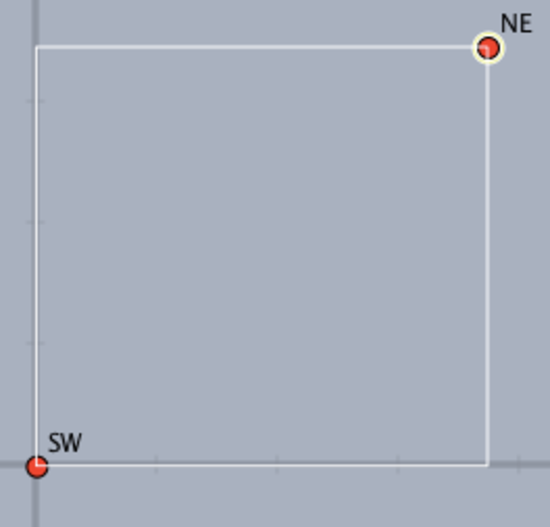
\includegraphics[bb=0.00 0.00 264.00 253.00,width=30mm]{fig/swne.pdf}}
\end{layer}

\begin{itemize}
\item
図のPDFをワードなどで使いたい\vspace{-2mm}
\item
描画領域 SW,NEで囲まれる長方形\\\vspace{-2mm}
\item
手順
1.Ketinitの直後に Setparent(ファイル名)\\
  "sankaku" 文字列\\
  Cdyname()+"p" Cindy名に"p"を追加\\
2.Windispg()の直前に Figpdf();\\
3.Figureの代わりにParentボタンを押す
\end{itemize}

\newslide{Texエディタのインストール}

\vspace*{18mm}

\slidepage
\begin{itemize}
\item
\TeX のエディタ\\
 ・編集とコンパイルと表示\\
 ・TeXWorks, TeXShop が一般的
\item
インストールと設定\\
 ・ ketcindy home/エディタ設定 を参照
\end{itemize}
%%%%%%%%%%%%

%%%%%%%%%%%%%%%%%%%%


\newslide{平面図形}

\vspace*{18mm}

\slidepage
\begin{itemize}
\item
Reference(以下Ref)のP13---33を参照
\item
主なコマンド\\
 Listplot, Lineplot, Circledata, Polygonplot, \\
 Pointdata, Arrowdata, Arrowhead\\
 Ellipseplot, Hyperbolaplot, Parabolaplot
\item
例\\
 \verb|Circledata("1",[A,B,C]);| A,B,Cを通る円\\
 \verb|Polygonplot("1",[A,B],8);| A中心の正8角形
\end{itemize}
%%%%%%%%%%%%

%%%%%%%%%%%%%%%%%%%%


\newslide{関数のグラフ}

\vspace*{18mm}

\slidepage

\begin{layer}{120}{0}
\end{layer}

\begin{itemize}
\item
RefのP33---39を参照
\item
主な関数\\
 Plotdata, Paramplot
\item
例\\
 \verb|Plotdata("1","sin(x)","x");|
\item
3番目は描画範囲(文字だけの場合は[XMIN,XMAX]);
\item
[課題]\monban log(x)のグラフを [0.01,XMAX]  で描け\\
 (スクリプトを答えよ)
\end{itemize}
%%%%%%%%%%%%

%%%%%%%%%%%%%%%%%%%%


\newslide{オプションとデータ名}

\vspace*{18mm}

\slidepage
\begin{itemize}
\item
Reference(以下Ref)のP11---12を参照
\item
コマンドの引数の最後に\verb|[ ]|をおく
\item
省略したらデフォルト値を使う\\
例)\verb|Listplot("1",[[p1,p2]],["dr,2","Color=red"]);|\\
例)\verb|Plotdata("2","sin(5*x)","x",["Num=200"]);|
\item
データの名前は,種別+最初の文字列\\
 上の例の場合のデータ名は sg1, gr2
\end{itemize}
%%%%%%%%%%%%

%%%%%%%%%%%%%%%%%%%%


\newslide{データの変換}

\vspace*{18mm}

\slidepage
\begin{itemize}
\item
RefのP53---56を参照
\item
主なコマンド\\
 Rotatedata, Scaledata, \\
 Translatedata, Reflectdata
\item
例)\verb|Rotatedata("sg1",pi/6);|\\
  \verb|Rotatedata("gr1",pi/6,[[1,2]]);|
\item
[課題]\monban 適当な図形を適当に変換してみよ.\\
 (スクリプトを答えよ)
\end{itemize}
%%%%%%%%%%%%

%%%%%%%%%%%%%%%%%%%%


\newslide{文字列の書き込み}

\vspace*{18mm}

\slidepage
\begin{itemize}
\item
RefのP39---41を参照
\item
主なコマンド\\
 Letter, Expr 文字列,数式をかく
\item
例) \verb|Letter(A,"se","A");| Aの南東に文字Aをかく\\
  \verb|Expr([2,3],"nw","\sin x");| [2,3]の北西に$\sin x$
\item
[課題]\monban 三角形ABCの頂点の座標を書き入れよ\\
 幾何点Aの座標は\verb|A.xy|\\
 リスト点p1のx座標は\verb|p1_1|
\end{itemize}
%%%%%%%%%%%%

%%%%%%%%%%%%%%%%%%%%


\newslide{シェードと斜線}

\vspace*{18mm}

\slidepage

\begin{layer}{120}{0}
\end{layer}

\begin{itemize}
\item
RefのP48---52を参照
\item
主な関数\\
 Hatchdata, Shade
\item
例\\
 \verb|Circledata("1",[A,2])| //Aは幾何点, 2は半径\\
 \verb|Hatchdata("1",["i"],[["cr1"]],[])|
\end{itemize}
%%%%%%%%%%%%

%%%%%%%%%%%%%%%%%%%%


\newslide{他の機能}

\vspace*{18mm}

\slidepage
\begin{itemize}
\item
今回は説明しない機能\\
 作表,多面体,曲面(Cが必要)
\item
layer環境
\item
KeTCindyJS
\end{itemize}
%%%%%%%%%%%%

%%%%%%%%%%%%%%%%%%%%


\newslide{授業後アンケート}

\vspace*{18mm}

\slidepage
\begin{itemize}
\item
[課題]\monban 次に答えてください\seteda{70}\\
\eda{\ketcindy の概要がわかりましたか}\\
\eda{授業の内容に興味を持てましたか}\\
\eda{特に面白かったことがあったら書いてください}\\
\eda{もっと知りたいことがあったら書いてください}
\end{itemize}
\label{pageend}\mbox{}

\end{document}
